%% LyX 2.0.8.1 created this file.  For more info, see http://www.lyx.org/.
\documentclass[english]{article}
\usepackage[T1]{fontenc}
\usepackage[utf8]{luainputenc}
\usepackage{amsmath}
\usepackage{graphicx}
\PassOptionsToPackage{normalem}{ulem}
\usepackage{ulem}

\makeatletter

%%%%%%%%%%%%%%%%%%%%%%%%%%%%%% LyX specific LaTeX commands.
%% Because html converters don't know tabularnewline
\providecommand{\tabularnewline}{\\}
%% A simple dot to overcome graphicx limitations
\newcommand{\lyxdot}{.}


%%%%%%%%%%%%%%%%%%%%%%%%%%%%%% User specified LaTeX commands.
\usepackage{cite}
\usepackage[T1]{fontenc}
\usepackage{inputenc}
\usepackage{authblk}

\makeatother

\usepackage{babel}
\begin{document}

\title{A genetic similarity measure for identifying fine-scale population
stratification and cryptic relatedness\author[1]{Daniel Schlauch} 
\author[1]{Christoph Lange}
\affil[1]{Department of Biostatistics and Computational Biology, Dana-Farber Cancer Institute and Department of Biostatistics, Harvard TH Chan School of Public Health, Boston, MA 02115}}
\maketitle
\begin{abstract}
The improving quality and falling costs of next-generation sequencing
has allowed for vast increases in availability of these data. With
this increased abundance comes a new ability to investigate population
structure with previously unattainable precision. In addition to the
anthroplogical value, properly accounting for confounding in GWAS,
particularly for rare variants, is of meaningful importance. {[}More
about rare variants, recent migration, relatedness, etc...{]}
\end{abstract}

\section*{Introduction}

The impact of confounding due to population structure and cryptic
relatedness is well established \cite{ptak2002evidence, pritchard2000association, roeder2009searching}.
Many approaches are utilized to address this concept at the analysis
level, such as PCA\cite{price2006principal,price2010new}, mixed models
\cite{listgarten2012improved,zhou2012genome,yang2014advantages,kang2010variance},
etc. or at the data collection level by limiting the scope of the
study to homogeneous populations or matching by ancestry. However,
as our ability to further detect structure increases with developing
methods and technologies we find that even supposedly homogeneous
populations contain detectable population structure that may inflate
type I error particularly among rare variants \cite{mathieson2012differential}.
Additionally, the presence on cryptic relatedness presents further
potential for confounding in GWAS, increasing both type I and type
II errors \cite{voight2005confounding, sun2012identifying,li2014relationship}.

Much of the structure identifcation improvement can be attributed
to our ability to identify rare alleles. Rare alleles may be exploited
due to the fact that they are more likely to have arisen recently
and thus a superior approach towards separating populations that have
recently separated\cite{mathieson2014demography}. Furthermore, very
low allele frequencies are more unstable than higher allele frequency,
either becoming fixed at zero or becoming more common with high probability. 

In this study we present a genetic similarity measure that is designed
to separate individuals with recent common ancestry. Our measure has
clearly defined properties which can be used to test for homogeneity
in a population and in particular identify individuals who are likely
be related in a study population.


\section*{Methods}

Exploiting the relative value of rare alleles is fundamental to our
method, which uses an intuitive, computationally straightforward approach
towards identfying similarity between two individuals. Effectively,
we give a larger weight to a genotype which is common to two individuals
if the allele frequency is low among the rest of the population.

For a matrix of $n$ individuals ($2n$ haploid genomes), with $N$
variants described by the genotype matrix $\mathbf{G}_{2n\times N}$,
we define the weighted Jaccard similarity between two haploid genomes,
$s_{i,j}$

\[
s_{i,j}=\frac{\sum_{k=1}^{N}w_{k}\mathbf{G}_{i,k}\mathbf{G}_{j,k}}{\sum_{k=1}^{N}I\left[\sum_{l=1}^{2n}\mathbf{G}_{l,k}>1\right]}
\]


where 

\[
w_{k}=\begin{cases}
\frac{{\sum_{l=1}^{2n}\mathbf{G}_{l,k} \choose 2}}{{2n \choose 2}} & \sum_{l=1}^{2n}\mathbf{G}_{l,k}>1\\
0 & \sum_{l=1}^{2n}\mathbf{G}_{l,k}\le1
\end{cases}
\]
\begin{align*}
E\left(s_{i,j}|\mbox{No structure}\right) & =1
\end{align*}


It therefore follows from the central limit theroem that in the absence
of populations structure, cryptic relatedness and dependence between
loci (such as linkage disequilibrium) the distribution of the test
statistic, $s_{i,j}$ is Gaussian.
\[
s_{i,j}\sim N\left(1,\sigma^{2}\right)
\]
Where $\sigma^{2}$ is estimated by 
\[
\hat{\sigma^{2}}=\hat{Var}\left(s_{i,j}|\mbox{No structure}\right)=\frac{\sum_{k=1}^{N}\hat{p}_{k}^{2}\left(1-\hat{p}_{k}^{2}\right)w_{k,i,j}^{2}}{\left(\sum_{k=1}^{N}I\left[\sum_{l=1}^{2n}\mathbf{G}_{l,k}>1\right]\right)^{2}}
\]


This provides an easily interpreted statistical test for evaluating
possible relatedness between individuals in a purportedly homogeous
dataset of unrelated individuals.

Furthermore, this measure is particularly sensitive for measuring
relatedness. Intuitively, we can imagine two subjects which have a
kinship coefficient, $\Phi$, indicating a probability of a randomly
chosen allele in each person being identical by descent (IBD). For
an allele which belongs to the one person, the probability of it belonging
to the related person is $\Phi+\left(1-\Phi\right)\times p$, where
$p$ is the allele frequency in the population. We can clearly see
that for rare alleles, such that $p$ is small compared to $\Phi$,
there will be a much larger relative difference in the probability
of shared alleles among related individuals ($\Phi>0$) compared to
unrelated individuals ($\Phi=0$). Given that our method weights more
highly these rarer alleles, there is increased sensitivity to detection
of relatedness.

Consider a coefficient of relatedness, $\Phi>0$,
\begin{align*}
E\left(s_{i,j}|\Phi,\mbox{No other structure}\right) & =\sum_{k=1}^{N}w_{k}\left(\Phi p_{k}+\left(1-\Phi\right)p_{k}^{2}\right)\\
 & >1
\end{align*}


For example, in an otherwise homogeneous population of unrelated individuals
an uncle-nephew relationship ($\Phi=.125$), with $MAF\sim Uniform\left(.01,.1\right)$
we can directly calculate the expectation of their similarity statistic,
$s_{i,j}$ 
\[
E\left(s_{i,j}|\Phi=.125,\mbox{No other structure}\right)\approx2.9
\]


This approach is easily generalized to the diploid scenario. A diploid
similarity score, $s_{diploid}$, is obtained by averaging each of
the four pairwise haploid $s_{haploid}$ scores between each person's
two haploid genotypes. For $N$ individuals, $2N$ genotypes per loci,
the similarity between individuals $i$ and $j$ is defined as

\[
s_{diploid,i,j}=\frac{\sum_{k=1}^{N}\left[w_{k}\mathbf{G}_{i_{1},k}\mathbf{G}_{j_{1},k}+w_{k}\mathbf{G}_{i_{1},k}\mathbf{G}_{j_{2},k}+w_{k}\mathbf{G}_{i_{2},k}\mathbf{G}_{j_{1},k}+w_{k}\mathbf{G}_{i_{2},k}\mathbf{G}_{j_{2},k}\right]/4}{\sum_{k=1}^{2N}I\left[\sum_{l=1}^{2n}\mathbf{G}_{l,k}>1\right]}
\]
where $\mathbf{G}_{i_{2},k}$ refers to the $2^{nd}$ genotype of
individual $i$ at locus $k$.

This formulation will have the same mean
\[
E\left[s_{diploid,i,j}\right]=1
\]
and assuming independence of each individual's haploid genomes, such
as in the absence of inbreeding,
\[
\hat{Var}\left(s_{diploid,i,j}|\mbox{No structure}\right)=\frac{\hat{Var}\left(s_{haploid,i,j}|\mbox{No structure}\right)}{4}
\]
 


\section*{Identification of relatedness in 1000GP data}

We applied our method to data from the 1000 Genomes Project \cite{10002015global, 10002012integrated},
a consortium...{[}{]}.

These populations were not identified to have cryptic relatedness
or had cryptic relatedness removed \textbf{{[}citation difficult (pptx
file posted online KGP website) ftp://ftp.1000genomes.ebi.ac.uk/vol1/ftp/phase1/analysis\_results/supporting/cryptic\_relation\_analysis/Nemesh\_crypticrelatedness\_20120213.pptx{]}}.

Phase 3 of the 1000 Genomes Project contains approximately 2504 individuals
with a combined total of 88 million variants. To test our method,
we sampled 80,000 variants uniformly spaced in the dataset in order
to limit the impact of linkage disequilibrium. Our method was then
run on each of the 26 populations in the study as well as on 5 super
populations and the study as a whole.

We discovered that there was great variation in the presence of cryptic
relatedness and population structure across the 26 populations of
the study. Under the assumptions that each study contained a homogeneous
population of unrelated individuals, only a handful of groups contained
neither large outliers nor heavily inflated numbers of significant
results.

We defined the presence of population structure as applying to those
populations which had a median $s_{i,j}<.97$. Using this criterion,
three of the 26 populations met this threshold- MXL (Mexican Ancestry
from Los Angeles USA), PUR (Puerto Ricans from Puerto Rico), and PEL
(Peruvians from Lima, Peru). Each of these populations are ``new
world'' populations which have undergone extensive admixture in the
past centuries. It is therefore unsurprising that these groups of
individuals would exhibit the greatest amount of heterogeneity among
the populations surveyed.

We defined the presence of cryptic relatedness as those individual
pairs which exceed the cutoff for a family-wise error rate of $\alpha=.01$.
Cryptic relatedness was discovered in 12 \textbf{{[}update this with
latest results{]}} of the 26 populations using this method. 

The overlap in these two groups may be due to the fact that the variance
in similarity is inflated in the presence of population structure.
So it is not accurate to identify cryptic relatedness in this manner
in popultations which contain structure. However, in populations which
do not exhibit detectable structure, we still find many instances
of related individuals in this study. For example, two individuals
from the ACB population (African Caribbeans in Barbados) had a $s_{i,j}$
score of $2.6$ $\left(p<10^{-30}\right)$, whereas no other pairing
exceeded the family-wise cutoff of 1.3 $\left(p=.0002\right)$. Using
the formula above, we estimate this relationship to be $\Phi=X$ {[}Redo
this analysis{]}, indicating...

\begin{figure}
\textbf{Distribution of similarity statistic within population subgroups
from 1000 Genomes Project }

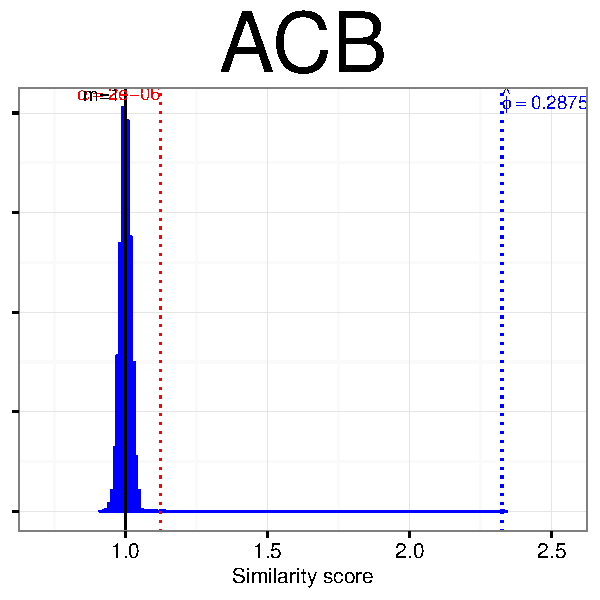
\includegraphics[width=0.1\paperwidth]{/home/dan/1000GP/plots/s_distributions/ACBdiploid}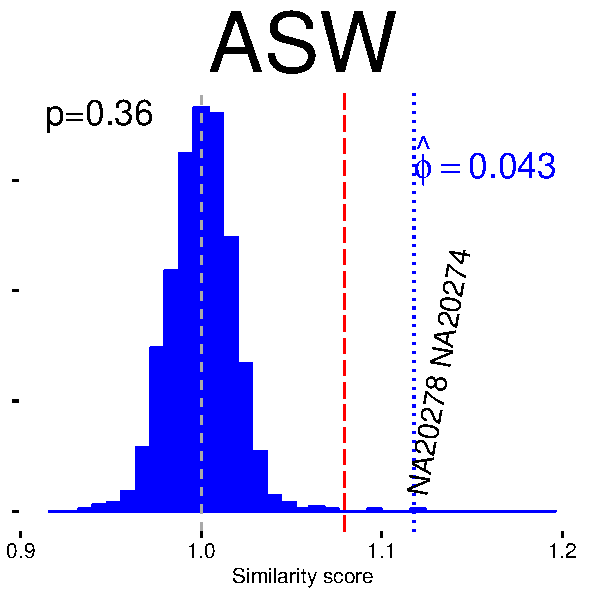
\includegraphics[width=0.1\paperwidth]{/home/dan/1000GP/plots/s_distributions/ASWdiploid}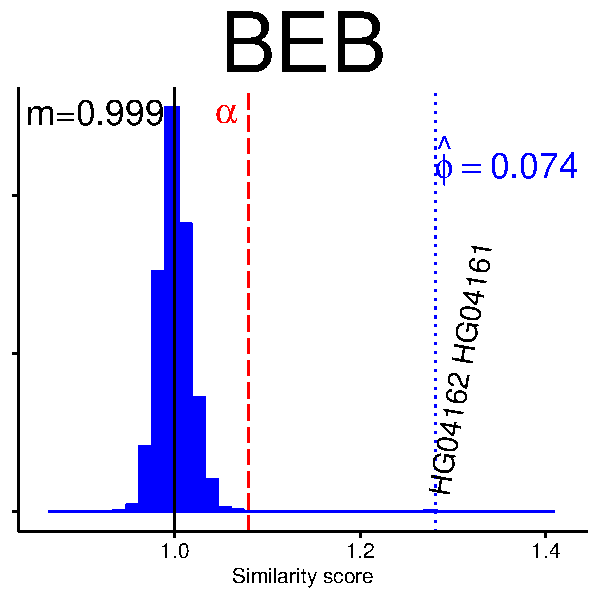
\includegraphics[width=0.1\paperwidth]{/home/dan/1000GP/plots/s_distributions/BEBdiploid}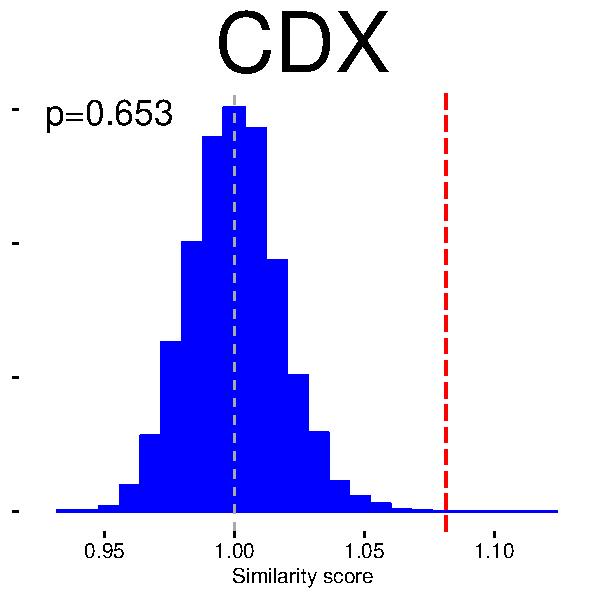
\includegraphics[width=0.1\paperwidth]{/home/dan/1000GP/plots/s_distributions/CDXdiploid}

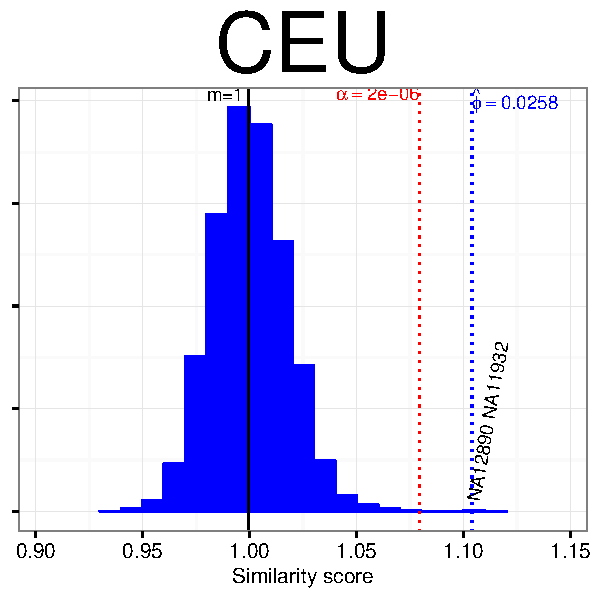
\includegraphics[width=0.1\paperwidth]{/home/dan/1000GP/plots/s_distributions/CEUdiploid}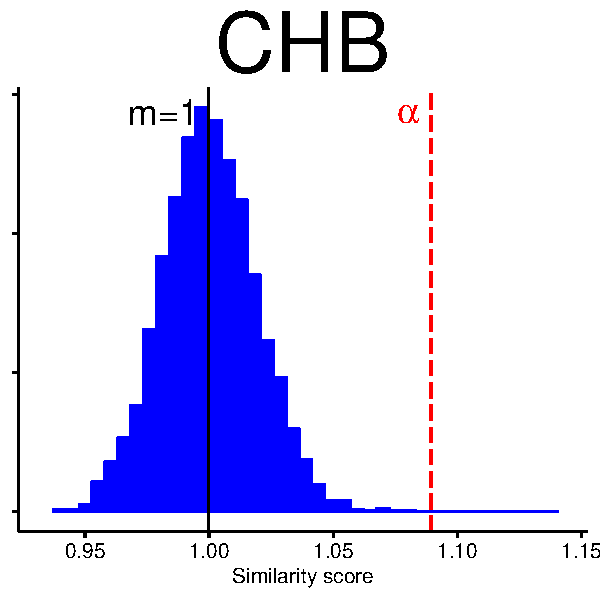
\includegraphics[width=0.1\paperwidth]{/home/dan/1000GP/plots/s_distributions/CHBdiploid}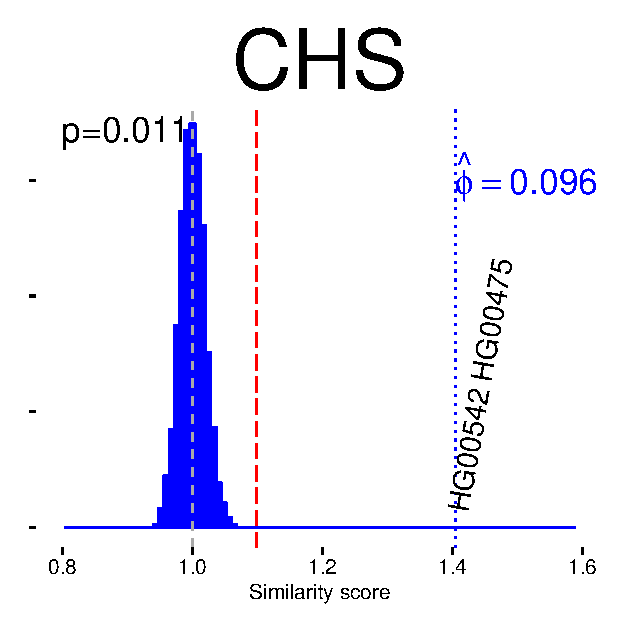
\includegraphics[width=0.1\paperwidth]{/home/dan/1000GP/plots/s_distributions/CHSdiploid}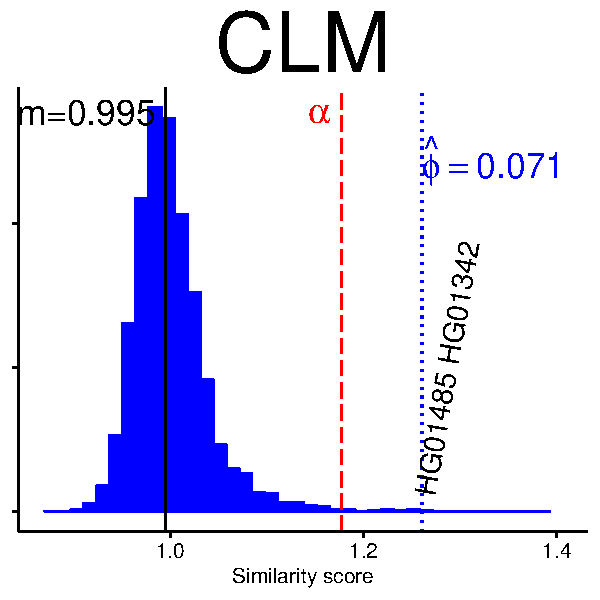
\includegraphics[width=0.1\paperwidth]{/home/dan/1000GP/plots/s_distributions/CLMdiploid}

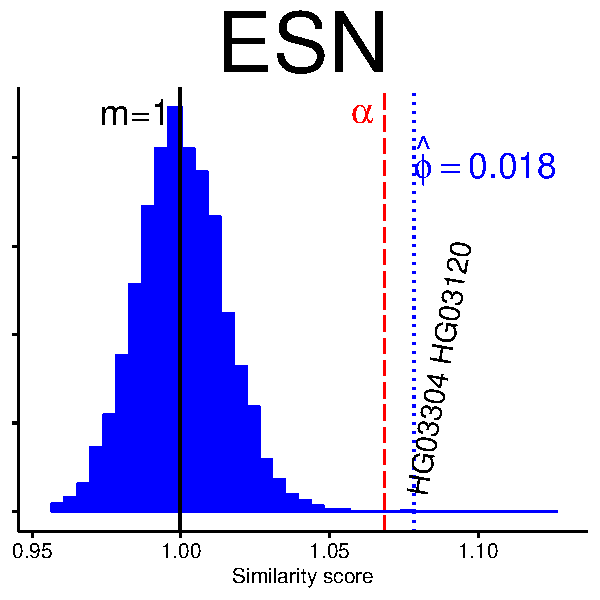
\includegraphics[width=0.1\paperwidth]{/home/dan/1000GP/plots/s_distributions/ESNdiploid}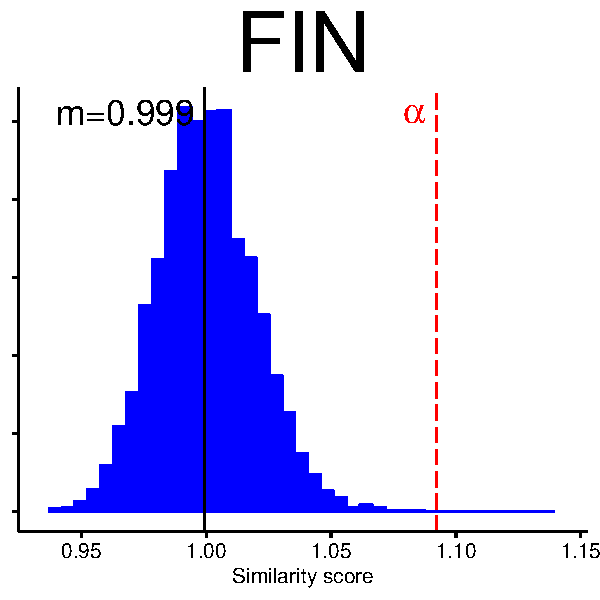
\includegraphics[width=0.1\paperwidth]{/home/dan/1000GP/plots/s_distributions/FINdiploid}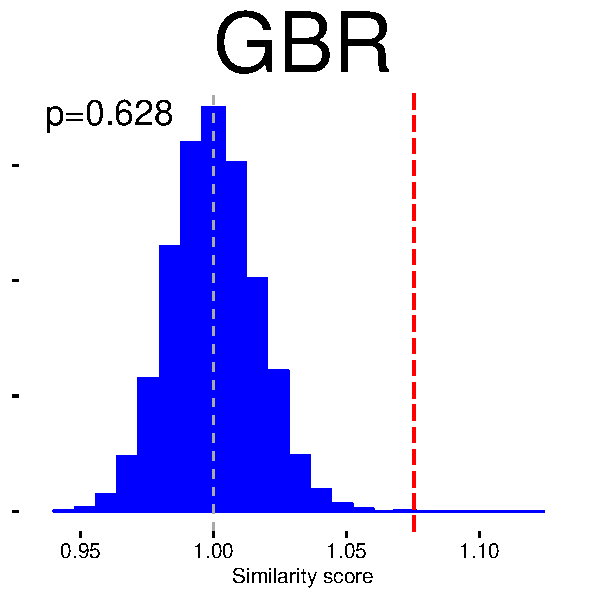
\includegraphics[width=0.1\paperwidth]{/home/dan/1000GP/plots/s_distributions/GBRdiploid}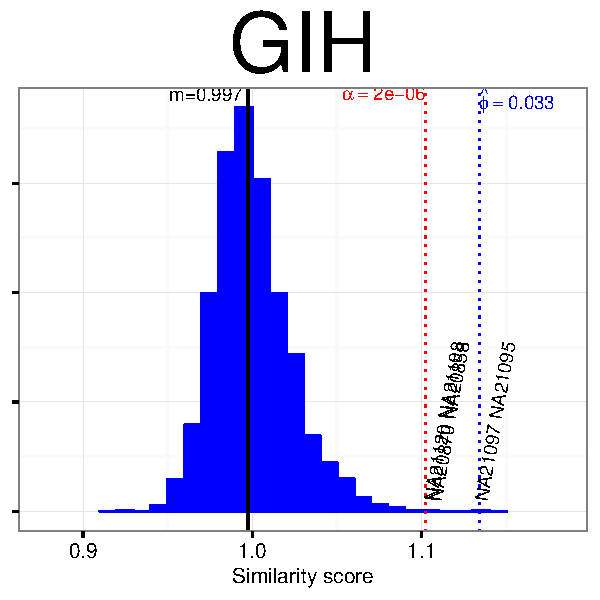
\includegraphics[width=0.1\paperwidth]{/home/dan/1000GP/plots/s_distributions/GIHdiploid}

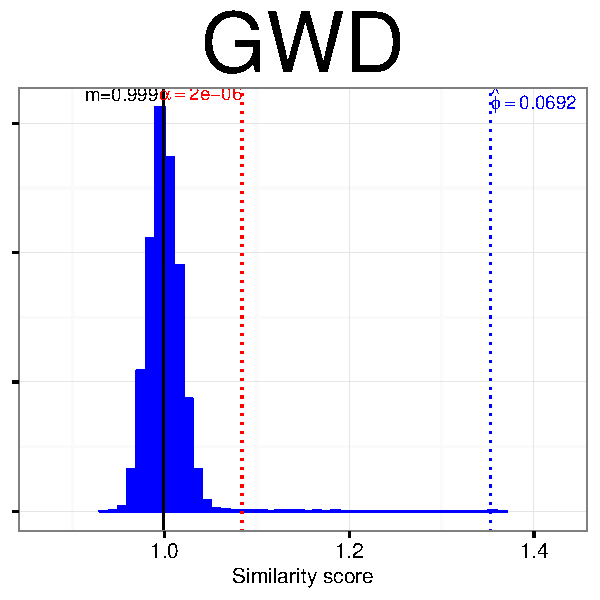
\includegraphics[width=0.1\paperwidth]{/home/dan/1000GP/plots/s_distributions/GWDdiploid}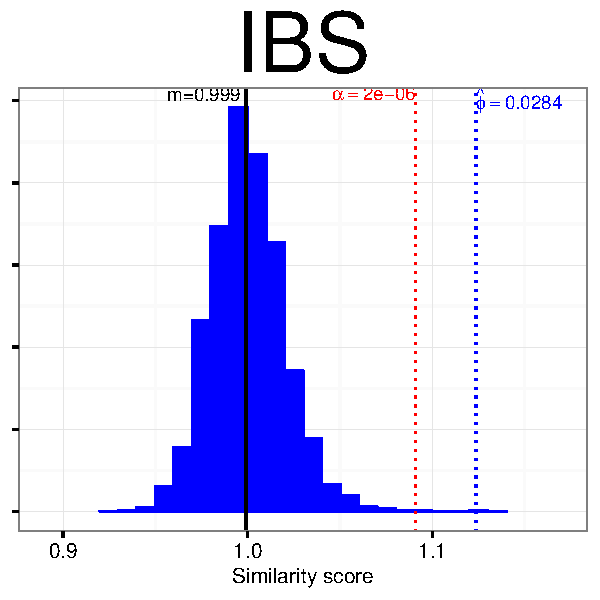
\includegraphics[width=0.1\paperwidth]{/home/dan/1000GP/plots/s_distributions/IBSdiploid}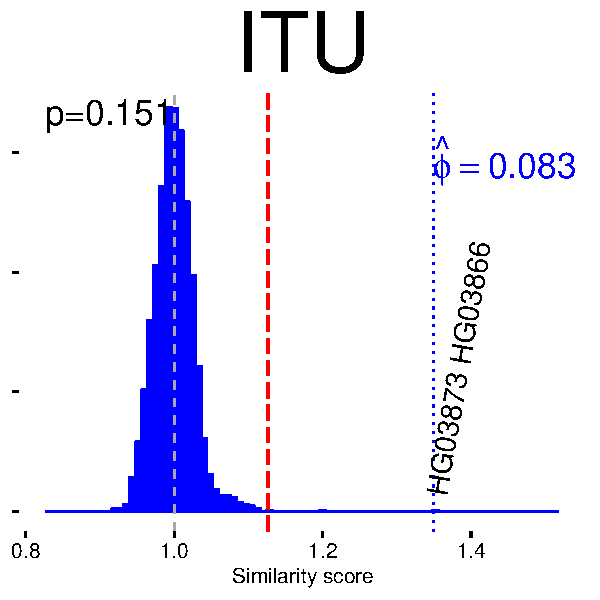
\includegraphics[width=0.1\paperwidth]{/home/dan/1000GP/plots/s_distributions/ITUdiploid}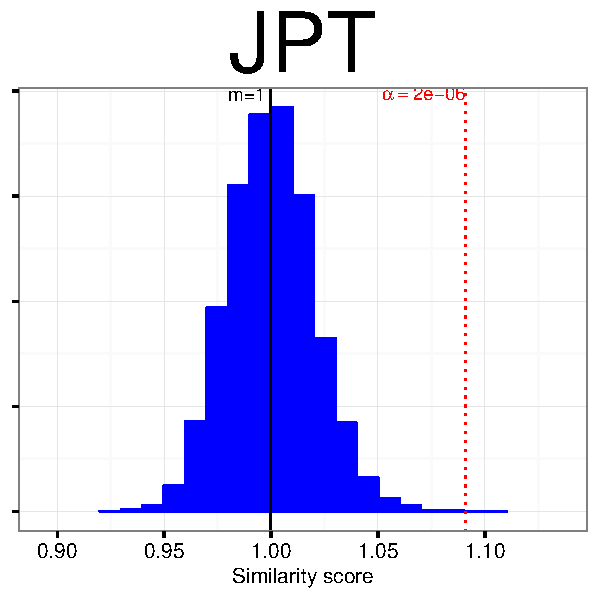
\includegraphics[width=0.1\paperwidth]{/home/dan/1000GP/plots/s_distributions/JPTdiploid}

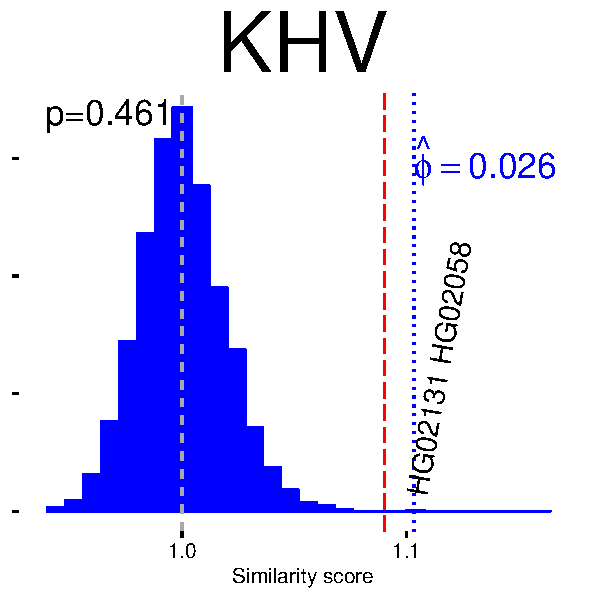
\includegraphics[width=0.1\paperwidth]{/home/dan/1000GP/plots/s_distributions/KHVdiploid}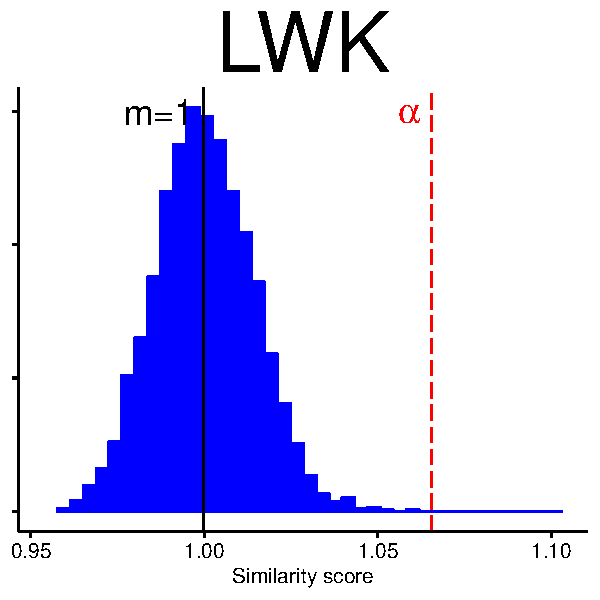
\includegraphics[width=0.1\paperwidth]{/home/dan/1000GP/plots/s_distributions/LWKdiploid}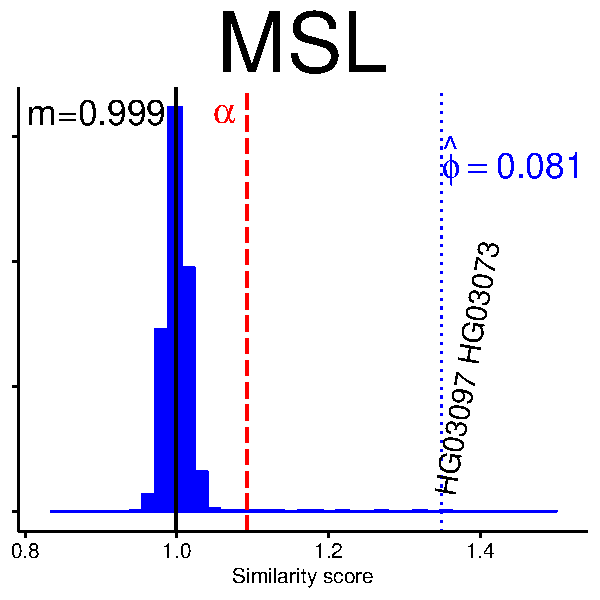
\includegraphics[width=0.1\paperwidth]{/home/dan/1000GP/plots/s_distributions/MSLdiploid}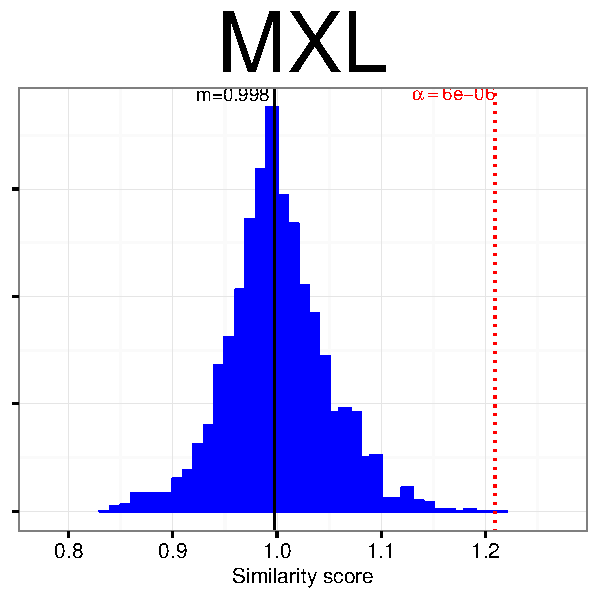
\includegraphics[width=0.1\paperwidth]{/home/dan/1000GP/plots/s_distributions/MXLdiploid}

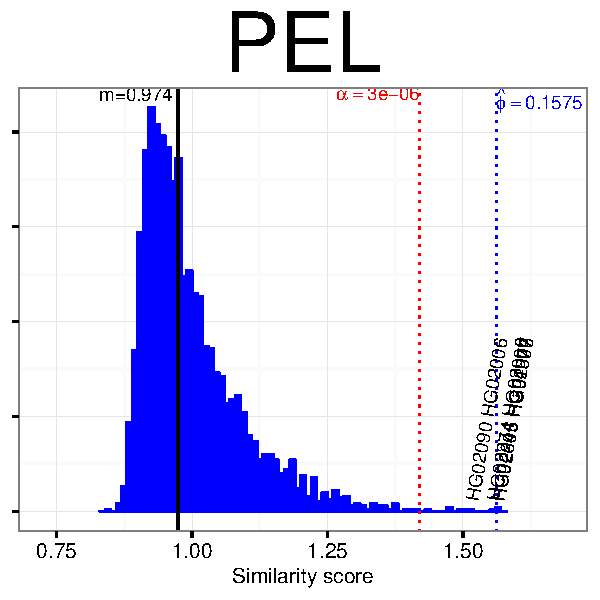
\includegraphics[width=0.1\paperwidth]{/home/dan/1000GP/plots/s_distributions/PELdiploid}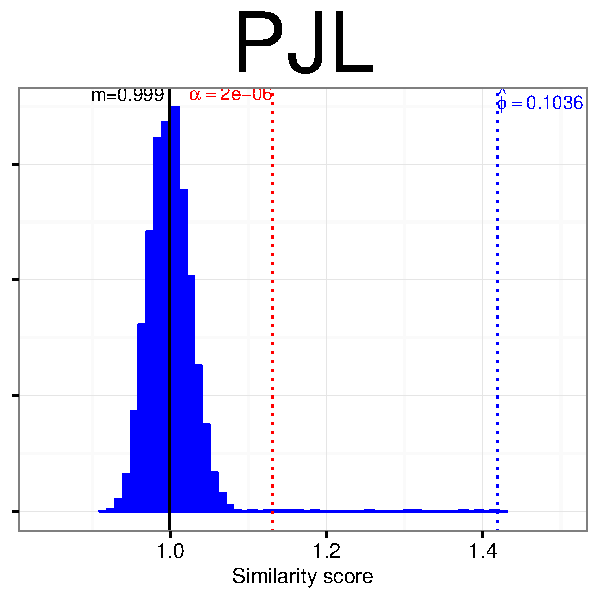
\includegraphics[width=0.1\paperwidth]{/home/dan/1000GP/plots/s_distributions/PJLdiploid}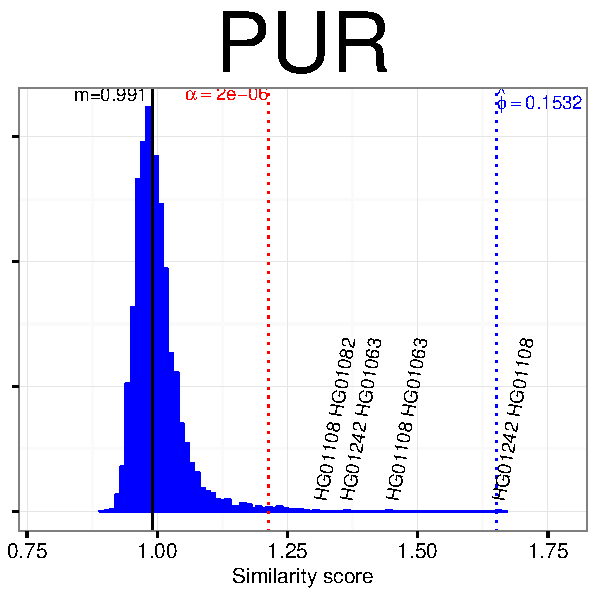
\includegraphics[width=0.1\paperwidth]{/home/dan/1000GP/plots/s_distributions/PURdiploid}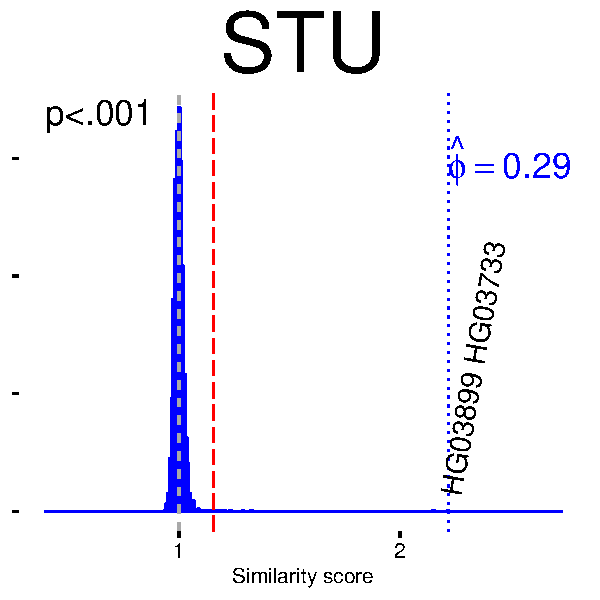
\includegraphics[width=0.1\paperwidth]{/home/dan/1000GP/plots/s_distributions/STUdiploid}

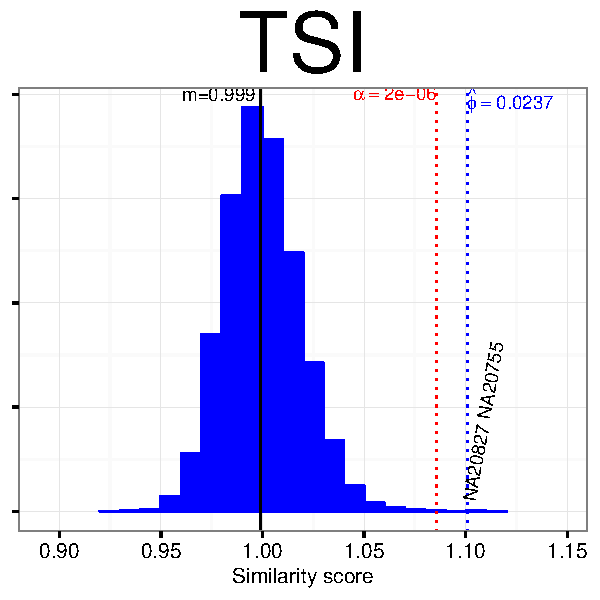
\includegraphics[width=0.1\paperwidth]{/home/dan/1000GP/plots/s_distributions/TSIdiploid}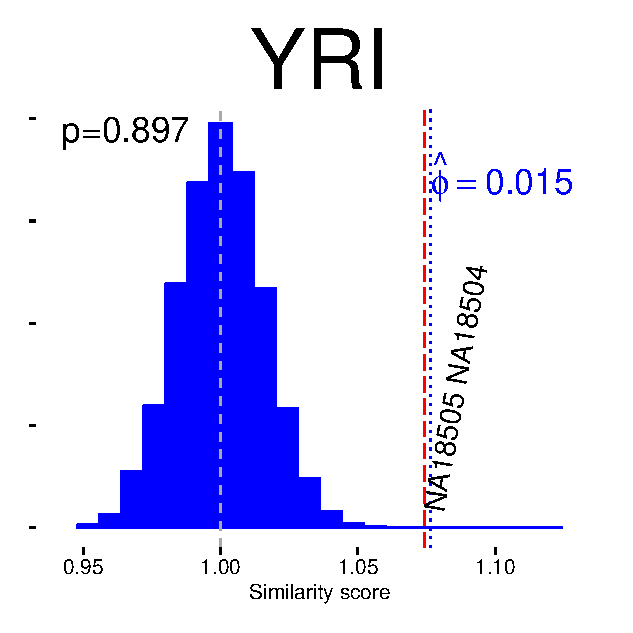
\includegraphics[width=0.1\paperwidth]{/home/dan/1000GP/plots/s_distributions/YRIdiploid}\caption{Distribution of similarity coefficients for each of the 26 populations
in the 1000 Genomes Project. Homogeneous populations lacking cryptic
relatedness should be expected to exhibit distributions centered around
1 with no outliers. The red dotted vertical line on each plot indicates
the family-wise$\alpha=.05$ level cutoff for ${n \choose 2}$ comparisons.
Many of the population groups do demonstrate the null behavior (e.g.
JPT, KHV, FIN)- however, a number of populations show the presence
of extreme outliers (e.g. STU, PUR) or systematic right skew (e.g.
MXL, PEL)}
\end{figure}
\begin{table}


\begin{tabular}{|c|c|c|}
\hline 
Population & Structure & Cryptic Relatedness\tabularnewline
\hline 
\hline 
ACB & No & Yes\tabularnewline
\hline 
ASW & No & Yes\tabularnewline
\hline 
BEB &  & \tabularnewline
\hline 
CDX & No & Maybe\tabularnewline
\hline 
CEU & No & No\tabularnewline
\hline 
CHB & No & No\tabularnewline
\hline 
CHS & No & Yes\tabularnewline
\hline 
CLM & No & No\tabularnewline
\hline 
ESN & No & Yes\tabularnewline
\hline 
FIN & No & No\tabularnewline
\hline 
GBR & No & No\tabularnewline
\hline 
GIH & No & Yes\tabularnewline
\hline 
GWD & No & No\tabularnewline
\hline 
IBS & No & No\tabularnewline
\hline 
ITU & No & Yes\tabularnewline
\hline 
JPT & No & No\tabularnewline
\hline 
KHV & No & No\tabularnewline
\hline 
LWK & No & Yes\tabularnewline
\hline 
MSL & No & Yes\tabularnewline
\hline 
MXL & Yes & Yes\tabularnewline
\hline 
PEL & Yes & No\tabularnewline
\hline 
PJL & No & Yes\tabularnewline
\hline 
PUR & Yes & Yes\tabularnewline
\hline 
STU & No & Yes\tabularnewline
\hline 
TSI & No & No\tabularnewline
\hline 
YRI &  & \tabularnewline
\hline 
\end{tabular}\caption{Presence of population structure and cryptic relatedness detected
in each of the 26 populations in the 1000 Genomes Project. Population
structure, defined as a $median\left(s\right)<.97$ was found in three
groups- MXL, PEL and PUR. Each of these populations are ``new world''
populations which have undergone extensive admixture in the past centuries.}


\end{table}



\section*{Population detection in 1000 Genomes Project}

There are many methods for detecting population structure. Most commonly,
Principal Components Analysis \cite{price2006principal,price2010new}is
applied for identifying the components of largest variation which
ideally corresponds to the population structure. This procedure first
involves the calculation of a genetic similarity matrix (GSM) via
the correlation between all samples, which is commonly followed by
an eigendecomposition of that matrix. There are a number of limitations
to this straightforward approach, one of which is that the calculation
of a variance-covariance matrix equally weights the impact of all
loci \textbf{{[}unless standardized by rows?{]}}, failing to fully
utilize the fact that the overall allele frequency is informative
of the value of each variant.

We used the 1000 Genomes Project data to compare the GSMs obtained
via the conventional variance-covariance matrix step and the use of
our method. We evaluated the ability of each method to separate the
same quantity of data into the 5 superpopulations and 26 populations.
Using approximately 80,000\textbf{ {[}Adjust for filtered{]}} variants,
we generated the two GSMs and plotted the similarity matrices, ordered
by hierarchical clustering with average linkage (Figure \ref{fig:heatmaps}).

Both methods performed well at separating the five superpopulations,
but the our method outperformed variance covariance in separating
populations of the same superpopulation. As expected, the lack of
focus on less frequent alleles, which are more important for distinguishing
recent ancestry allowed variance-covariance to adequately separate
continental origins, but failed to sufficiently partition the samples
according to subgroups.

\begin{figure}
\textbf{A}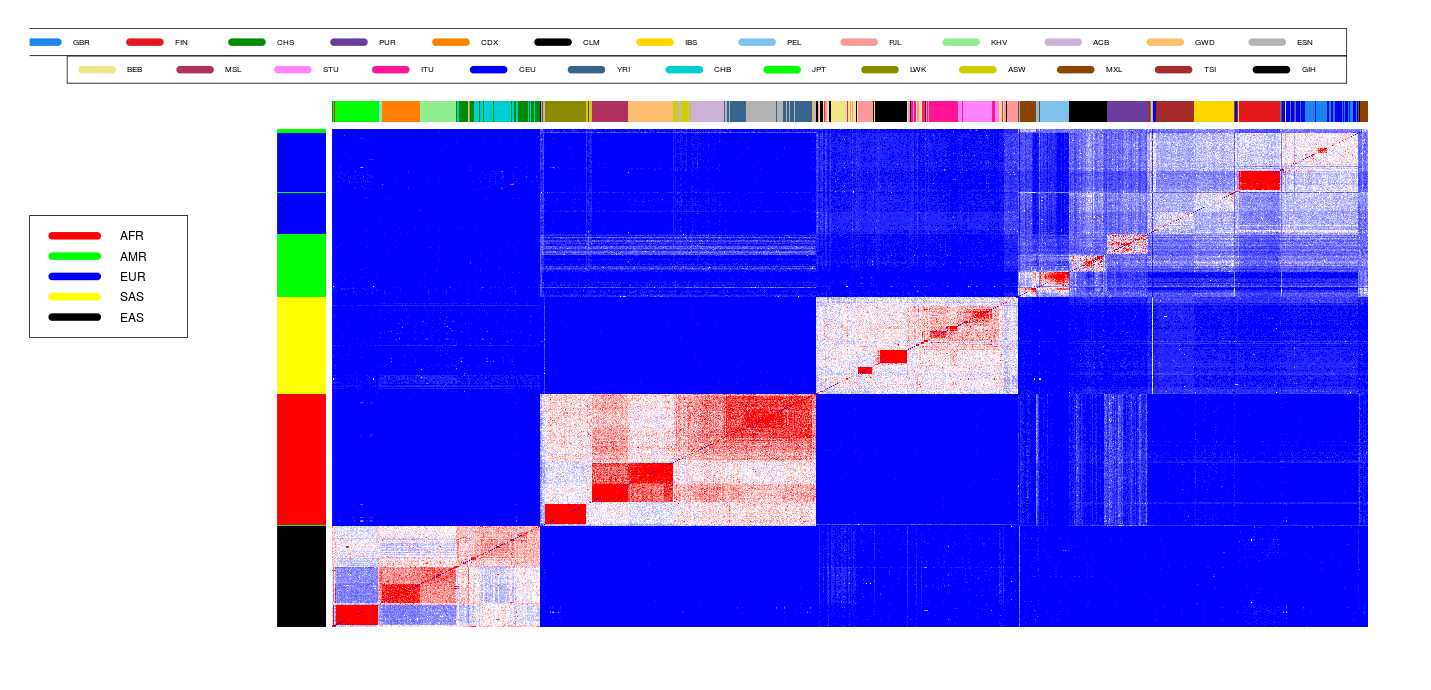
\includegraphics[width=0.5\columnwidth]{/home/dan/gd/Harvard/Research/R_workspace/Slides/pasted14}\textbf{B}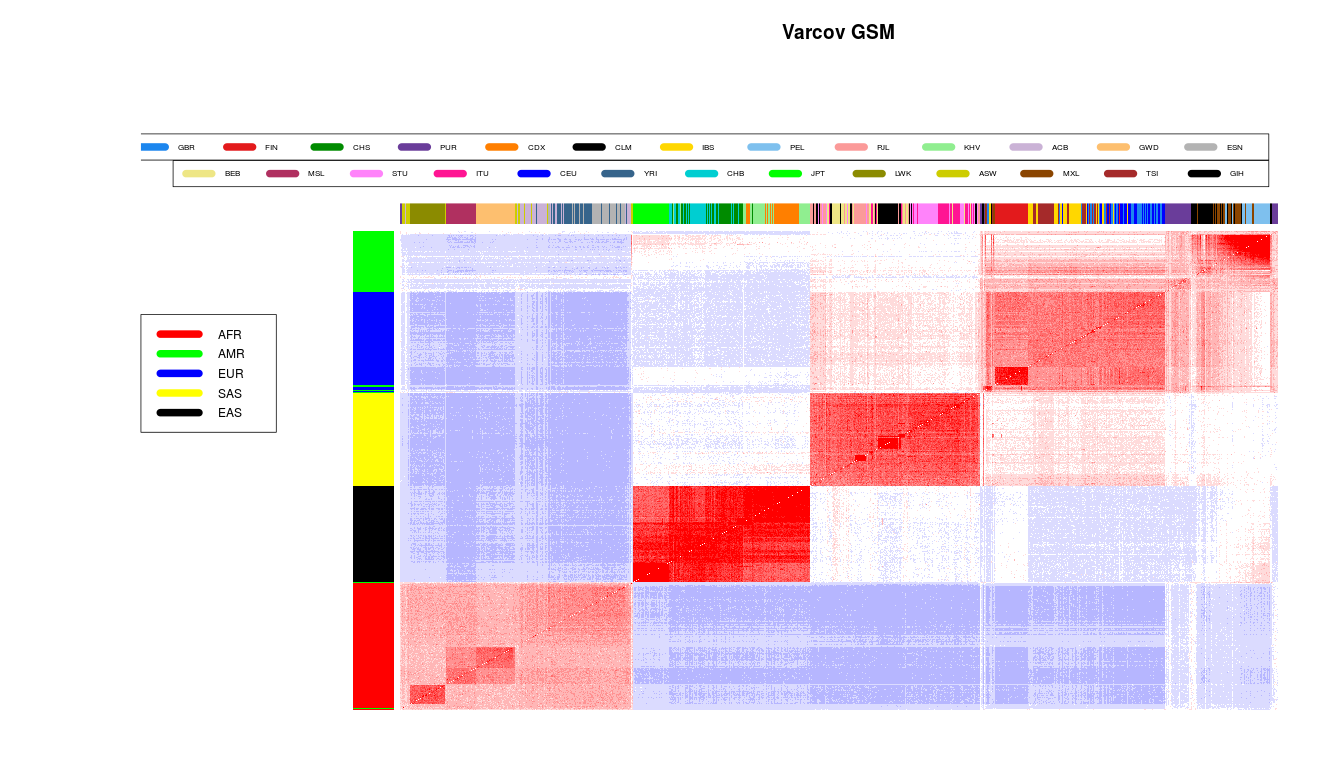
\includegraphics[width=0.5\columnwidth]{/home/dan/gd/Harvard/Research/R_workspace/Slides/pasted15}

\textbf{C}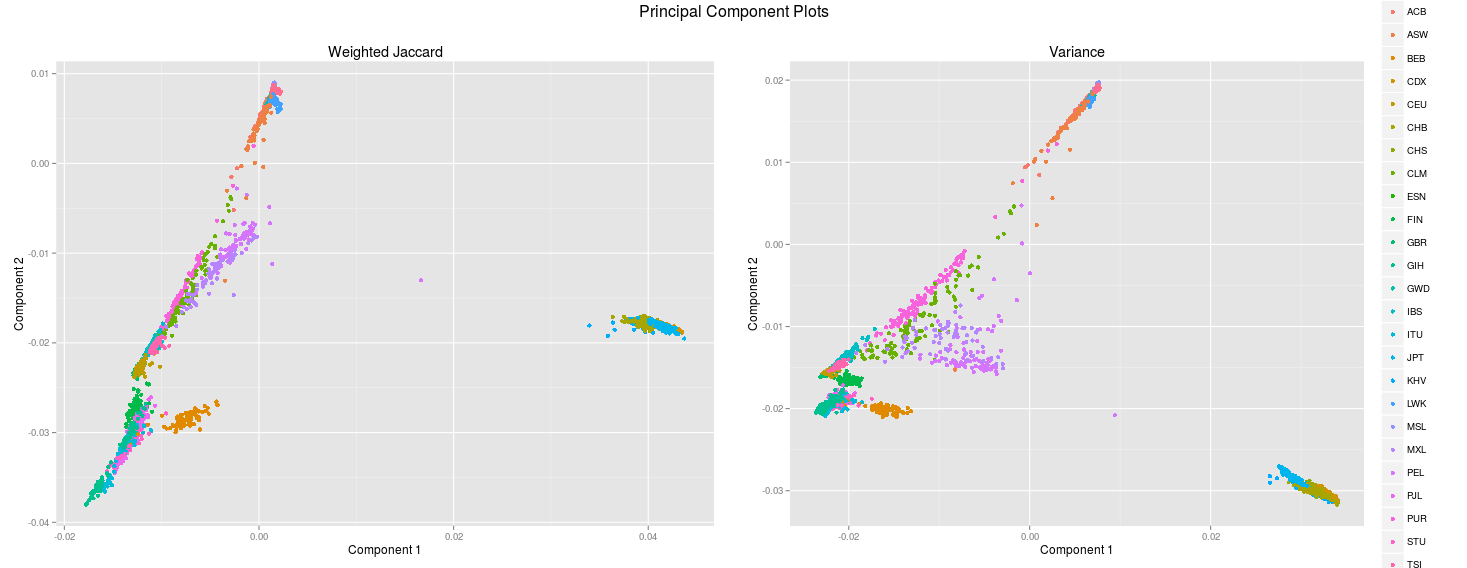
\includegraphics[width=1\columnwidth]{/home/dan/gd/Harvard/Research/R_workspace/Slides/pasted5}\caption{Heatmap of GSM generated by our method (A) and variance-covariance
(B) using 80,000 uniformly spaced variants. Samples have been ordered
by hierarchical clustering (dendrogram no shown). The vertical colorbar
indicates membership in one of the five superpopulations, while the
horizontal colorbar indicates membership in one of the 26 populations.
(C) Projecting each individual onto the top two eigenvectors resulted
in a similar 2-dimensional distribution of global ancestry}
\label{fig:heatmaps}
\end{figure}


The first two eigenvectors of the GSMs generated using our method
vs variance-covariance yield very similar results. Both methods provide
a sufficient separation of coarse-scale population structure. But
closer examination of fine-scale population structure reveals our
method to be an improvement over variance-covariance. We were able
to provide a stronger separation of all 26 populations, particularly
those of recent ancestry. As an example, we explored two populations-
Sri Lankan Tamil and Indian Telugu, which have relatively small geographical
separation.

Interestingly, we found a strong case for cryptic relatedness between
three pairs of individuals, one pair of which (HG03998 and HG03873)
spanned the two populations. Considering that both groups were sampled
in the UK, this suggests a distant genetic relationship is possible
from members of different population groups.

\begin{figure}
\textbf{A}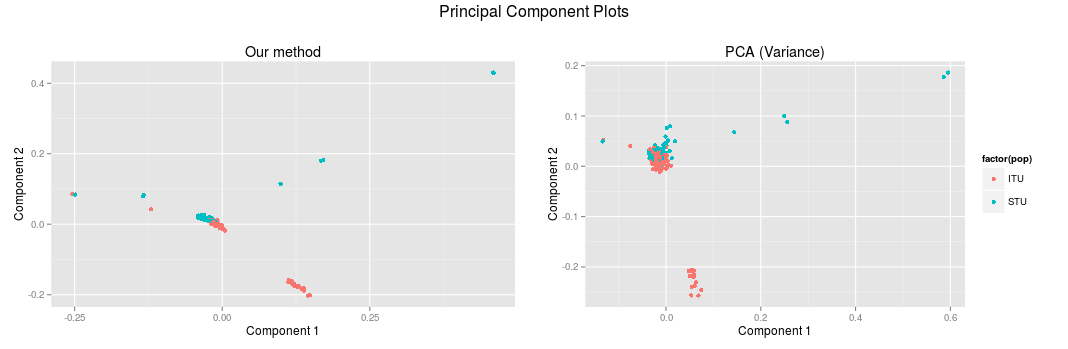
\includegraphics[width=0.6\columnwidth,height=0.3\paperheight,keepaspectratio]{/home/dan/gd/Harvard/Research/R_workspace/Slides/pasted23}

\textbf{B}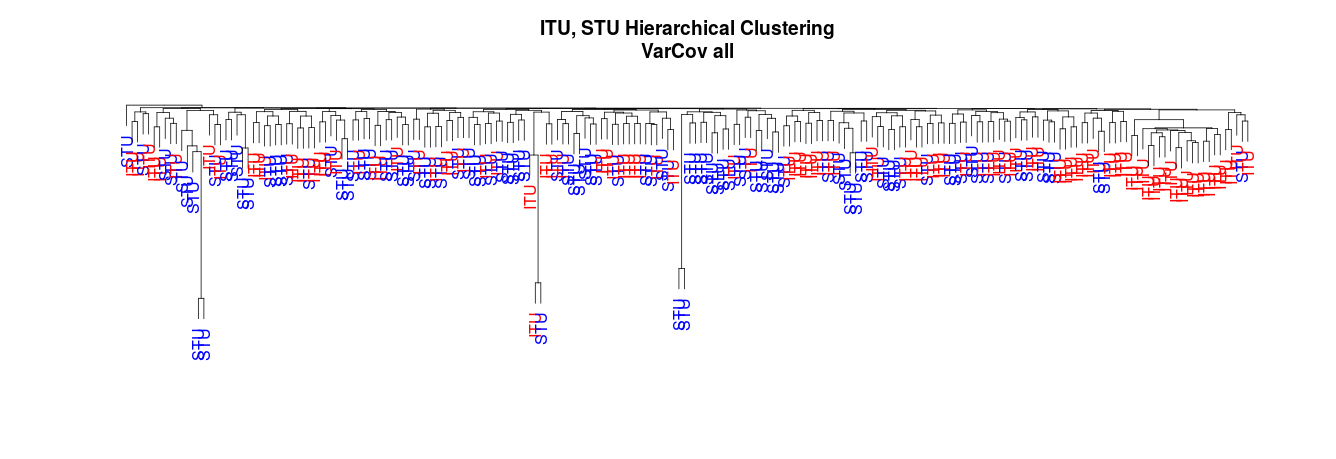
\includegraphics[width=0.4\columnwidth,height=0.2\paperheight,keepaspectratio]{/home/dan/gd/Harvard/Research/R_workspace/Slides/pasted30}

\textbf{C}\includegraphics[width=0.4\columnwidth,height=0.2\paperheight,keepaspectratio]{\string"/home/dan/1000GP/plots/hcl_ ITU vs STU/P0-0.4\string".png}

\textbf{C}\includegraphics[width=0.6\columnwidth]{/home/dan/1000GP/plots/s_distributions/ITU_STUdiploid}

\textbf{{[}Rerun this figure on whole dataset{]}}\caption{\textbf{Example: ITU vs STU}. Two populations of Southern Asian origin,
Indian Telugu from the UK (ITU) and Sri Lankan Tamil from the UK (STU)
show poor separation using the variance-covariance approach. When
using our method, we see improved separation of populations when individuals
are projected onto the top two eigenvectors (\textbf{A}) despite the
fact that our method appears to have expended a greater proportion
of the variance explanation on identification of related individuals.
Hierarchical clustering using the GSM as a similarity matrix (\textbf{B})
was unable to clearly visually distinguish between ITU and STU, but
use of our method provided much clearer results (\textbf{C}). }
\label{fig:heatmaps}
\end{figure}



\section*{Rarer alleles are more informative for recent ancestry}

\begin{figure}
\textbf{A}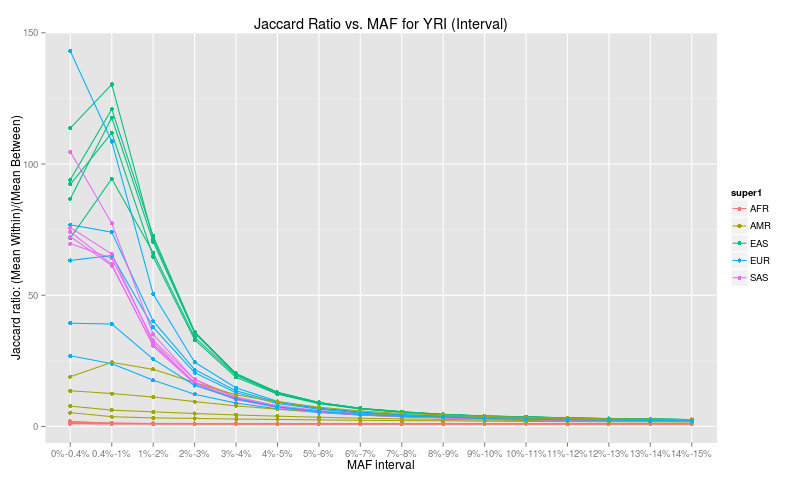
\includegraphics[width=0.5\columnwidth]{/home/dan/gd/Harvard/Research/R_workspace/Slides/pasted13}\textbf{B}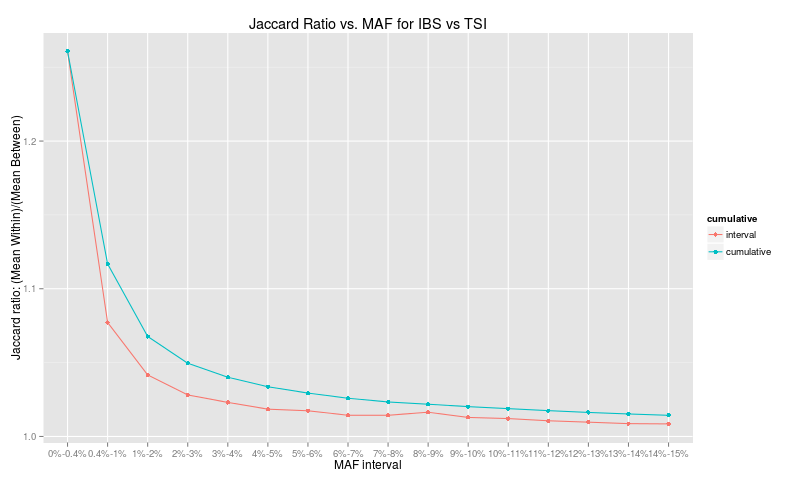
\includegraphics[width=0.5\columnwidth]{/home/dan/gd/Harvard/Research/R_workspace/Slides/pasted7}\caption{(\textbf{A}) Ratio for mean within-population jaccard ratio vs mean
out-of-population jaccard ratio for Yoruba in Ibadan, Nigeria (YRI)
compared to all other populations. We find that in comparising YRI
to all other populations, the within-population vs out-of-population
ratio increases as the allele frequency decreases. This trend held
true for all 26 populations. For the smallest allele frequency bin,
0\%-0.4\%, the trend is not as clear suggesting that this is the point
at which quality control is of concern when considering rare variants.
(\textbf{B}) Ratio for mean within-population jaccard ratio vs mean
out-of-population jaccard ratio for two populations with a relatively
recent common ancestry- Iberian Population in Spain (IBS) and Toscani
in Italia (TSI). Although the ratio is unsurprisingly on a smaller
scale, we find that the most informative variants are those with the
smallest allele frequency.}
\end{figure}



\section*{More figure and text, not sure where this goes}

Separation of recent shared ancestries

{\tiny Example:
Indian Telugu from the UK (ITU) 
Sri Lankan Tamil from the UK (STU)}

\begin{figure}
\includegraphics[width=0.8\paperwidth,height=0.2\paperheight,keepaspectratio]{\string"/home/dan/1000GP/plots/hcl_ ITU vs STU/F9-10\string".png}\includegraphics[width=0.8\paperwidth,height=0.2\paperheight]{\string"/home/dan/1000GP/plots/hcl_ IBS vs TSI/P0-0.4\string".png}\includegraphics[width=0.8\paperwidth,height=0.2\paperheight]{\string"/home/dan/1000GP/plots/hcl_ IBS vs TSI/F9-10\string".png}

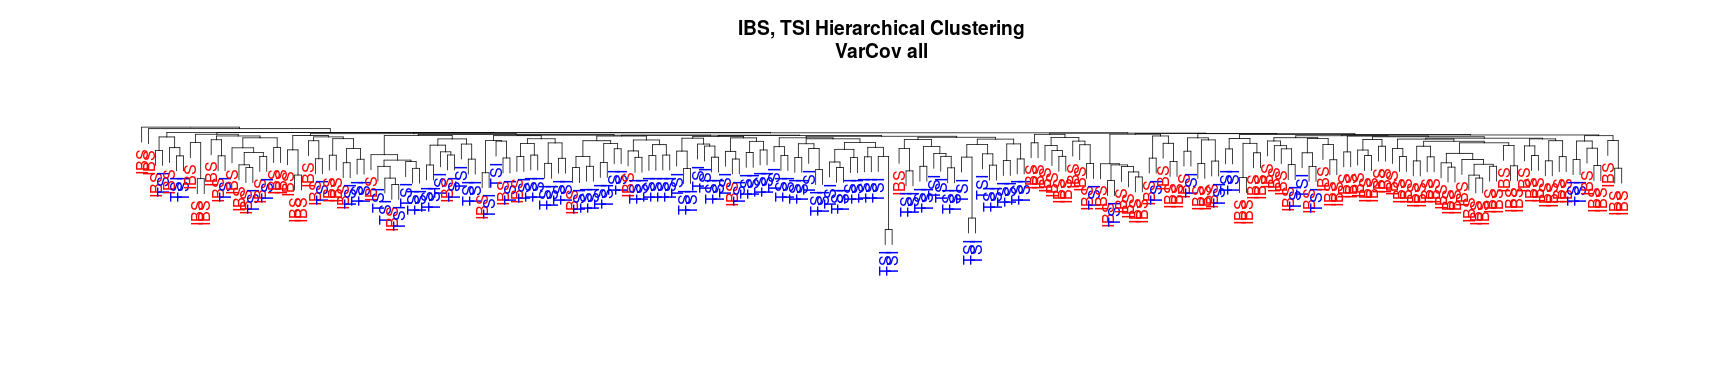
\includegraphics[width=0.8\paperwidth,height=0.2\paperheight]{/home/dan/gd/Harvard/Research/R_workspace/Slides/pasted32}\caption{Figures...}
\end{figure}


Separation of recent shared ancestries

{\tiny Example:
Iberian Population in Spain (IBS)
Toscani in Italia (TSI)}

Separation of recent shared ancestries

Ratio of within-group mean distance to out-of group mean distance:

\begin{tabular}{|c||c|c|}
\hline 
\multicolumn{1}{|c|}{Populations} & Our method & PCA\tabularnewline
\hline 
\hline 
TSI-IBS & .417 & .504\tabularnewline
\hline 
BEB-PJL & .748 & .794\tabularnewline
\hline 
ITU-STU & .836 & .889\tabularnewline
\hline 
ITU-BEB & .905 & .951\tabularnewline
\hline 
CHB-CHS & .605 & .681\tabularnewline
\hline 
LWK-ESN & .178 & .197\tabularnewline
\hline 
GIH-ITU & .513 & .552\tabularnewline
\hline 
CEU-YRI & .025 & .022\tabularnewline
\hline 
\end{tabular}

Our method outperformed standard PCA in differentiating groups for
\emph{\uline{every}} same-continent subpopulation pairing across
all continents. ($\approx50$ comparisons)


\section*{dddd}

The Mathieson paper (Nature Genetics, 2012) proposed a problem wherein
the case of sharply spatially defined phenotypic risk lead to the
inflation of association test statistics for rare variants. Moreover,
this effect was not resolved using existing methods for controlling
for confounding by population stratification. The Listgarten response
(Listgarten et al, Nature Genetics 2012) claimed to solve this with
their novel method LMM-select. This method effectively uses a linear
mixed model approach but rather than use all variants to generate
their genetic similarity matrix, selects only those which are correlated
with phenotype. A more recent paper on which Listgarten was an author
(Widmer, Further Improvements…, Nature 2014), appears to reverse this
claim. In this paper, Widmer admits one potential improvement, building
a GSM based on selected SNPs that well predict the phenotype failed
rather dramatically. In particular, when population structure, family
relatedness, or both were present, this approach failed to control
for type I error. Seemingly indicating that their group’s previous
claim was premature. However, they claim now that inclusion of principal
components as fixed effects does properly control for type I error.
{[}However, I don’t see it demonstrated in the paper and I remain
somewhat unclear skeptical about what definition they are using{]}.
(For example, we are focusing on extreme events, where inflation is
only measurable at $\approx10^{-6}$)

A possible explanations for the test statistic inflation was suspected
to be primarily due to lack of a precise measure of genetic similarity.
This was attributed in part due to the fact that linear methods such
as PCA would have difficulty expressing sharply defined risk regions.

However, we found that test statistic inflation persisted even when
controlling for the exact regions for which we simulated differential
phenotypic risk. This demonstrated that although proper estimation
of the genetic similarity matrix is necessary, it is not sufficient
to control type I error. As we show here, association tests in the
presence of properly controlled population stratification exhibit
overdispersion due to the existence of high leverage individuals after
adjusting for confounding. 

A consistent estimator of rare-allele association in stratified GWAS
We developed a statistic which is asymptotically unbiased by calculating
the variance of the observed squared correlation statistic in the
presence of differential variance for both spatially-adjusted genotypes
and spatially-adjusted phenotypes. Intuitively, with uniform variance
across samples (such as with no population stratification) we expect
the variance of the correlation to be asymptotically $\sqrt{\frac{1}{n}}$.
In this case, we have the Armitage Trend Test statistic- $n\times r^{2}\sim\chi_{1}^{2}$.
However, in the presence of adjusted population stratification the
variance of the observed correlation is not $\sqrt{\frac{1}{n}}$.
Depending on whether the correlation of the variances of adjusted
genotypes and adjusted phenotypes are positive or negative we see
that the variance of the observed correlation is greater than or less
than sqrt(1/n), respectively. Insert derivation here

In combination with our estimated test statistic, we propose a method
for estimating the GSM by using the Jaccard Similarity Index (JSI)
for alleles which are present in less than 2\% of the population.
Our method is motivated by the plausible expectation that rare alleles
are more likely to have emerged most recently in human ancestral history
and thus may be superior differentiators for groups which have a more
recent ancestral divergence. An eigendecomposition of the JSI-GSM
can then be used to to identify linear predictors of ancestry in a
manner similar to Principal Components Analysis.

Jaccard Index vs Variance-Covariance approach. Use of Jaccard similarity
for rare alleles only in estimating GSM outperformed the standard
variance covariance approach.

Computation of the JSI for all pairs is computationally faster than
the more commonly used variance-covariance method typically employed
for PCA (maybe the same speed?)

Use of JSI provides clearer separation of closely related subpopulations
The ability to separate distinct subpopulations with a recent shared
ancestry, such as Spanish (IBS) and Italians (TSI), is a desirable
goal in GWAS. Even with $F_{ST}$ values smaller than $.001$, there
is a clear bias when performing GWAS on non-genetic outcomes correlated
with phenotype. The ability to separate closely related populations
was found to be a function of the allele frequency interval.

Separation of Sri Lankan and Indian populations using the Jaccard
Similarity and based on a global allele frequency of <0.4\% (top)
compared to a global allele frequency of \textasciitilde{}15\% (bottom)

The plot above shows the relative ability to separate two closely
related populations based on the allele frequency used. We see a monotonically
decreasing separation score as more common alleles are used indicating
that the ancestry informativeness peaks when utilizing the rarest
loci. We find that the estimated ratio of mean within-group JSI to
between group JSI is maximized by excluding all but those alleles
with <.04\% MAF and that inclusion of higher frequency alleles reduces
our ability to differentiate low Fst populations. Additionally, we
find that although rare alleles may outperform more common alleles
for closely related populations the use of a higher cutoff for more
distant populations may be appropriate. This could be attributed to
a relatively greater sensitivity to quality control issues for groups
which already have a clear genetic separation at higher allele frequencies.
The plot below demonstrates the increased efficacy of less common
alleles in separating Yoruban persons (YRI) from those populations
from other continental origins. The Jaccard ratio drops at the lowest
allele frequency interval, possibly due to the presence of randomly
miscalled genotypes.


\section*{Simulations}

We used real genotype data and simulated non-genetic phenotypes based
on reported population membership in the 1000 Genomes Project. ...describe
details of simulations...

estimator is consistent estimator is biased estimator is superior
to rare-PCA -how to quantify?

Argue: is estimator superior to usual PCA? estimator is equivalent
to subpopulation label?

\bibliographystyle{plain}
\bibliography{publications}

\end{document}
